\section{Amiral Technologies, une start-up prometteuse}
\subsection{Description de l'entreprise}
Amiral Technologies est une start-up spécialisée dans le développement et le développement du logiciel de prédiction de pannes, Diagfit.
Dérivée (spin-off) du CNRS, l'entreprise participe activement à la recherche dans le domaine de la science des données (datascience) et de l'intelligence artificielle.

Fondée en 2018, elle compte actuellement 22 employés et cible principalement trois secteurs d'activité : les transports (entreprises ferroviaires et aéronautiques), l'industrie manufacturière (dans le cadre de l'industrie 4.0) et le secteur de l'énergie et du nucléaire.

\subsection{Une entreprise dans un marché exigeant}
\subsubsection{Les entreprises clientes}
Reconnu pour la qualité du logiciel Diagfit, plusieurs clients de renom ont fait appel à l’expertise d’Amiral Technologies afin d'améliorer leur programme de maintenance de leurs équipements.

La start-up s'oriente vers trois secteurs précis pour canaliser leur communication : le secteur des transports avec les entreprises ferroviaires et aéronautiques, le secteur manufacturier en aidant le développement d'une industrie 4.0 et le secteur de l'énergie et du nucléaire.

\begin{figure}[ht!]
    \begin{minipage}[c]{0.33\textwidth}
        \hspace{10px}
\includegraphics[width=0.8\textwidth]{paper/figures/sncf.pdf}
    \end{minipage}
    \begin{minipage}[c]{0.5\textwidth}
        \hspace{10px}
\includegraphics[width=0.8\textwidth]{paper/figures/mersen.pdf}
    \end{minipage}

    \begin{minipage}[c]{0.5\textwidth}
        \hspace{10px}
\includegraphics[width=0.8\textwidth]{paper/figures/thales.pdf}
    \end{minipage}
    \begin{minipage}[c]{0.5\textwidth}
        \hspace{10px}
\includegraphics[width=0.8\textwidth]{paper/figures/airbus.pdf}
    \end{minipage}
    \vspace{5px}
    \caption{Entreprises clientes d'Amiral Technologies}
    \label{fig:clients}
\end{figure}

\newpage

\subsubsection{Le logiciel Diagfit}
Il permet aux équipements industriels de fonctionner sans défaut et sans pannes en anticipant les problèmes potentiels grâce à l'analyse de données de capteurs.

DiagFit utilise des modèles d'apprentissage automatique qui le rendent exploitable par une personne sans connaissances (réalité physique des capteurs et datascience).
L'un des atouts majeurs de DiagFit est sa capacité à traiter une multitude d'équipements différents de manière polyvalente, ce qui le rend adaptable à diverses industries.
Enfin, le logiciel utilise une méthode d'apprentissages efficace avec seulement 3h de données de capteurs dans un mode de fonctionnement sain.
Pour promouvoir l'adoption de Diagfit, il est crucial de souligner que l'outil permet d'éviter les pannes coûteuses en industrie.
Il n'est pas nécessaire de générer des pannes pour obtenir des résultats significatifs lors de l'apprentissage du logiciel Diagfit.

\begin{figure}[ht!]
    \centering
    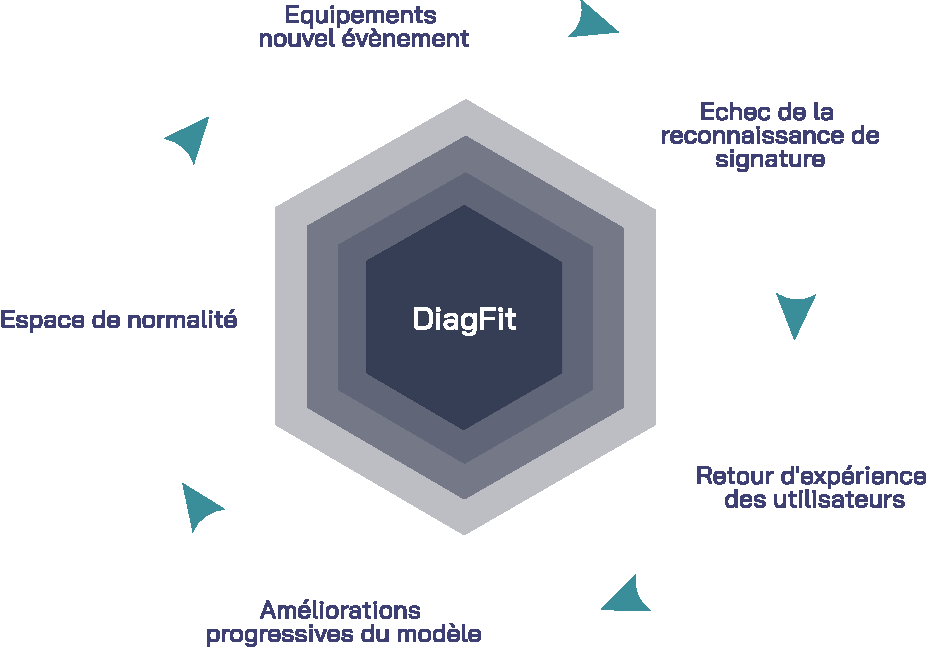
\includegraphics[width=0.6\textwidth]{paper/figures/diagfit.pdf}
    \caption{Évolution du logiciel Diagfit}
    \label{fig:diagfit}
\end{figure}

La détection de pannes permet d'entreprendre des maintenances prédictives en fonction des données spécifiques à l'appareil en question et non à une moyenne de la classe de ces appareils.
Cette technologie permet alors de réduire les coûts de maintenance en les consacrant uniquement lorsqu'elles sont nécessaires.

L'algorithme qui soutient le logiciel Diagfit est crucial pour l'entreprise, et d'importants efforts sont déployés pour préserver sa confidentialité.
Il constitue la pierre angulaire de la startup, lui offrant un avantage distinctif sur le marché des startups de prédiction de pannes.

\subsection{Organisation interne}
\subsubsection{Une organisation en synergie pour l'innovation}
L'entreprise basée en Isère dans la ville de Grenoble est remarquée dans les salons spécialisés de Lyon et de Paris.

Voici un aperçu des membres clés de l'administration :
\begin{itemize}
    \item \textbf{Katia Hilal} : Présidente et co-fondatrice de l'entreprise, Katia apporte une expertise essentielle dans la vision stratégique de l'entreprise.
    \item \textbf{Mazen Alamir} : Co-fondateur d'Amiral Technologies et directeur de recherches au CNRS, Mazen est le créateur de l'algorithme derrière Diagfit.
    \item \textbf{Simon Gazikian} : Directeur général, Simon joue un rôle crucial dans le développement des partenariats et dans l'orientation globale d'Amiral Technologies.
    \item \textbf{Sebastien Le Gall} : En tant que directeur technique, Sebastien est responsable de la supervision et du développement de l'aspect technique du logiciel DiagFit et assure également une gestion efficace des opérations quotidiennes de l'entreprise.
\end{itemize}

\begin{figure}[ht!]
    \centering
    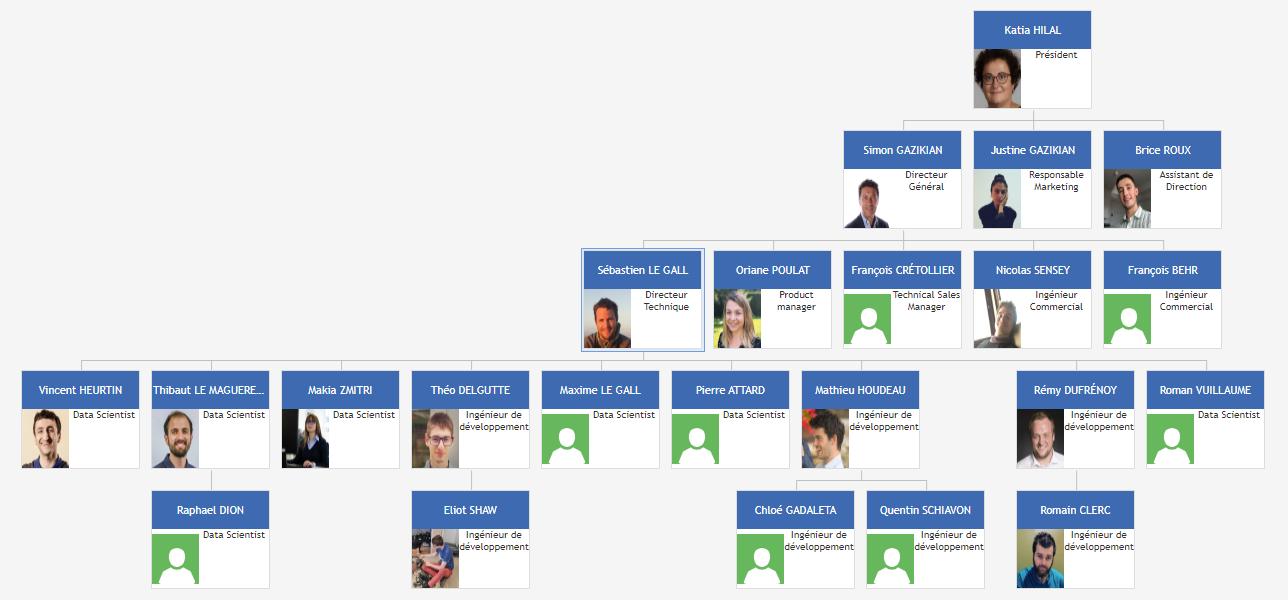
\includegraphics[width=0.95\textwidth]{paper/figures/orga.png}
    \caption{Organigramme de l'entreprise}
    \label{fig:organigramme}
\end{figure}

\newpage

Amiral Technologies est composé de différentes équipes en synergie pour pouvoir imaginer un algorithme, le développer en un logiciel et le vendre à de nombreux clients.

Description des groupes qui composent Amiral Technologies:
\begin{itemize}
    \item \textbf{L'équipe commerciale :} Responsable de l'identification et de l'établissement de partenariats avec les entreprises clientes pour promouvoir et vendre DiagFit.
    \item \textbf{Les data-scientists :} Experts en analyse de données, ils utilisent DiagFit pour interpréter les informations collectées par les capteurs et améliorer les prédictions de pannes.
    \item \textbf{Les développeur d'interface utilisateur (front-end) :} Chargés de concevoir et de développer l'interface utilisateur intuitive et conviviale de DiagFit.
    \item \textbf{Les développeurs côté serveur (back-end)} Responsables de la conception et du développement des fonctionnalités principales de DiagFit, en garantissant une performance optimale et une intégration harmonieuse des données.
    \item \textbf{Les administrateurs système :} Gèrent les infrastructures et s'assurent que le logiciel DiagFit fonctionne de manière sécurisée et fiable.
\end{itemize}

\subsubsection{Engagement envers la Responsabilité Sociétale des Entreprises}
\todo{resensement fait et vote des employés}
\todo{y aller moins fort 2e paragrapge}
\todo{et passage au parquet ensysteme de stockage}
\todo{fresque du climat}
\hyperref[rse]{La responsabilité sociétale des entreprises (RSE) est définie par la commission européenne comme l'intégration volontaire par les entreprises de préoccupations sociales et environnementales à leurs activités commerciales et leurs relations avec les parties prenantes.
En d'autres termes, la RSE est la contribution des entreprises aux enjeux du développement durable. [2]}

Amiral Technologies s'engage dans la Responsabilité Sociétale des Entreprises (RSE) en mettant en place des initiatives pour réduire son impact environnemental.
Cependant, certains choix peuvent être critiqués, notamment en ce qui concerne l'utilisation d'outils numériques de signature électronique qui génèrent une charge de stockage, ou l'investigation de l'empreinte carbone de l'entreprise sans exploitation des résultats.
Malgré cela, l'entreprise continue de rechercher des solutions durables pour améliorer sa contribution à la RSE.

La RSE est devenue un sujet crucial dans le monde des affaires, reflétant l'intérêt croissant des entreprises à contribuer positivement à la société et à l'environnement.
Dans la plupart des entreprises, les initiatives mises en œuvre pour répondre aux attentes en matière de RSE ont un fort accent sur le pilier écologique.
Cependant, une approche globale de la RSE nécessite également de considérer les autres piliers du développement durable, à savoir le pilier social et économique.
Des efforts peuvent être renforcés pour promouvoir le bien-être des employés, favoriser l'inclusion et l'équité dans le lieu de travail, ainsi que pour soutenir l'économie locale.

En tant que futur professionnel, il est essentiel d'être conscient de l'importance de la RSE et des trois piliers du développement durable.
C'est en contribuant d'une manière volontaire et naturelle que les entreprises pourront jouer un rôle réel dans la société.

